% ===========================
% Ultimate Scribe Template
% Tailored for Optimization / ML / Math Theory
% ===========================
\documentclass[11pt]{article}

% ---------------------------
% Encoding & typography
% ---------------------------
\usepackage[T1]{fontenc}
\usepackage[utf8]{inputenc}
\usepackage{lmodern}

% ---------------------------
% Page layout
% ---------------------------
\usepackage{geometry}
\geometry{margin=1in}

% ---------------------------
% Math packages
% ---------------------------
\usepackage{amsmath,amssymb,amsfonts,amsthm}
\usepackage{mathtools}
\usepackage{bm}              % bold math symbols
\usepackage{bbm}             % indicator function
\usepackage{physics}         % optional: \norm, \abs, \grad, etc. (can remove if undesired)

% ---------------------------
% Graphics / plots (optional)
% ---------------------------
\usepackage{graphicx}
\usepackage{tikz}
\usepackage{pgfplots}
\pgfplotsset{compat=1.18}

% ---------------------------
% Algorithms
% ---------------------------
\usepackage{algorithm}
\usepackage{algorithmic}

% ---------------------------
% Lists and tables
% ---------------------------
\usepackage{enumitem}
\usepackage{booktabs}

% ---------------------------
% Hyperlinks and clever references
% ---------------------------
\usepackage[colorlinks=true,linkcolor=blue,citecolor=blue,urlcolor=blue]{hyperref}
\usepackage[nameinlink]{cleveref}

% ---------------------------
% Notes / TODOs (optional)
% ---------------------------
\usepackage{todonotes}

% ---------------------------
% Colored boxes
% ---------------------------
\usepackage[most]{tcolorbox}

% ---------------------------
% Header / footer
% ---------------------------
\usepackage{fancyhdr}
\pagestyle{fancy}
\fancyhf{}
\lhead{\textsc{\CourseCode}: \CourseName}
\chead{\qquad Lecture \LectureNumber}
\rhead{\LectureDate}
\cfoot{\thepage}

% ---------------------------
% Custom commands: course metadata
% ---------------------------
\newcommand{\CourseCode}{26:711:685}
\newcommand{\CourseName}{Optimization Methods for ML}
\newcommand{\LectureNumber}{01}
\newcommand{\LectureTitle}{Lecture Title}
\newcommand{\LectureDate}{January 23, 2026}
\newcommand{\ScribeName}{Nilava Metya}
\newcommand{\InstructorName}{Mert G\"urb\"uzbalaban}

% ---------------------------
% Math shorthand (edit freely)
% ---------------------------
\newcommand{\R}{\mathbb{R}}
%\newcommand{\E}{\mathbb{E}}
\newcommand{\Prob}{\mathbb{P}}
\newcommand{\1}{\mathbbm{1}}
\newcommand{\argmin}{\operatorname*{arg\,min}}
\newcommand{\argmax}{\operatorname*{arg\,max}}
\newcommand{\Lip}{\operatorname{Lip}}

% Optimization operators
\newcommand{\prox}{\operatorname{prox}}
\newcommand{\diam}{\operatorname{diam}}
\newcommand{\dist}{\operatorname{dist}}

% ---------------------------
% Theorem environments
% ---------------------------
\theoremstyle{plain}
\newtheorem{theorem}{Theorem}[section]
\newtheorem{lemma}[theorem]{Lemma}
\newtheorem{proposition}[theorem]{Proposition}
\newtheorem{corollary}[theorem]{Corollary}

\theoremstyle{definition}
\newtheorem{definition}[theorem]{Definition}
\newtheorem{assumption}[theorem]{Assumption}
\newtheorem{example}[theorem]{Example}

\theoremstyle{remark}
\newtheorem{remark}[theorem]{Remark}

% Proof sketch environment
\newtheorem*{proofsketch}{Proof sketch}

% ---------------------------
% Box styles
% ---------------------------
\tcbset{
  sharp corners,
  boxrule=0.8pt,
  colback=white,
  colframe=black!60,
  left=1mm,right=1mm,top=1mm,bottom=1mm
}

\newtcolorbox{keyidea}{
  colback=blue!4!white,
  colframe=blue!70!black,
  title=Key idea
}
\newtcolorbox{intuition}{
  colback=cyan!3!white,
  colframe=cyan!60!black,
  title=Intuition
}
\newtcolorbox{warningbox}{
  colback=red!4!white,
  colframe=red!70!black,
  title=Warning / common pitfall
}
\newtcolorbox{complexitybox}{
  colback=green!4!white,
  colframe=green!60!black,
  title=Complexity summary
}
\newtcolorbox{assumptionsbox}{
  colback=yellow!6!white,
  colframe=yellow!50!black,
  title=Standing assumptions
}
\newtcolorbox{notationbox}{
  colback=gray!6!white,
  colframe=gray!60!black,
  title=Notation
}
\newtcolorbox{takeawaybox}{
  colback=purple!4!white,
  colframe=purple!70!black,
  title=Takeaways
}

% ---------------------------
% Lecture header macro
% ---------------------------
\newcommand{\LectureHeader}{
  \begin{center}
    {\Large \textbf{\CourseCode: \CourseName}}\\[2mm]
    {\large \textbf{Lecture \LectureNumber: \LectureTitle}}\\[2mm]
    \textbf{Date:} \LectureDate \qquad
    \textbf{Instructor:} \InstructorName \qquad
    \textbf{Scribe:} \ScribeName
  \end{center}
  \vspace{2mm}
  \hrule
  \vspace{4mm}
}
\input{../macro.tex}

% ===========================
% DOCUMENT
% ===========================
\begin{document}

\LectureHeader

% ---------------------------
% Quick overview (recommended)
% ---------------------------
\begin{keyidea}
We set up notation for optimization and study basics of level sets. We study one example of regression. This leads to the idea of level sets, `convexity', positive definiteness and gradient descent.
\end{keyidea}
% ===========================
% MAIN CONTENT
% ===========================

\section{Introduction to optimization}
We write $$\min_{x\in \cX}f(x)$$ to denote an optimization problem where $x$ is a decision variable, $f(x)$ is the objective (cost) function to minimize, $\cX$ is the constriant set. If a point $x_{*}$ that minimizes $f$ then we call it an \textit{optimizer} and $f(x_{*})$ is the \textit{optimal value}.  

\section{Simple Regression (one predictor)}

Let $y$ be the output variable (house prices), $a$ be the input vector and $x$ is the decision variable. The loss function we consider is $L(x,y,a) = \frac12(y-(x_{1}+x_{2}a_{1}))^{2}$. 

Example: Say I have a dataset with $(y,a)$ as $\set{(0,0),(1,1)}$. The loss becomes $f(x) = L(x,0,0)+L(x,1,1) = \frac{x_{1}^{2} + \left[ 1-(x_{1}+x_{2}) \right]^{2}}2$. This $f(x)=0$ looks like a `cereal bowl'.
\begin{figure}[h]
 \centering
  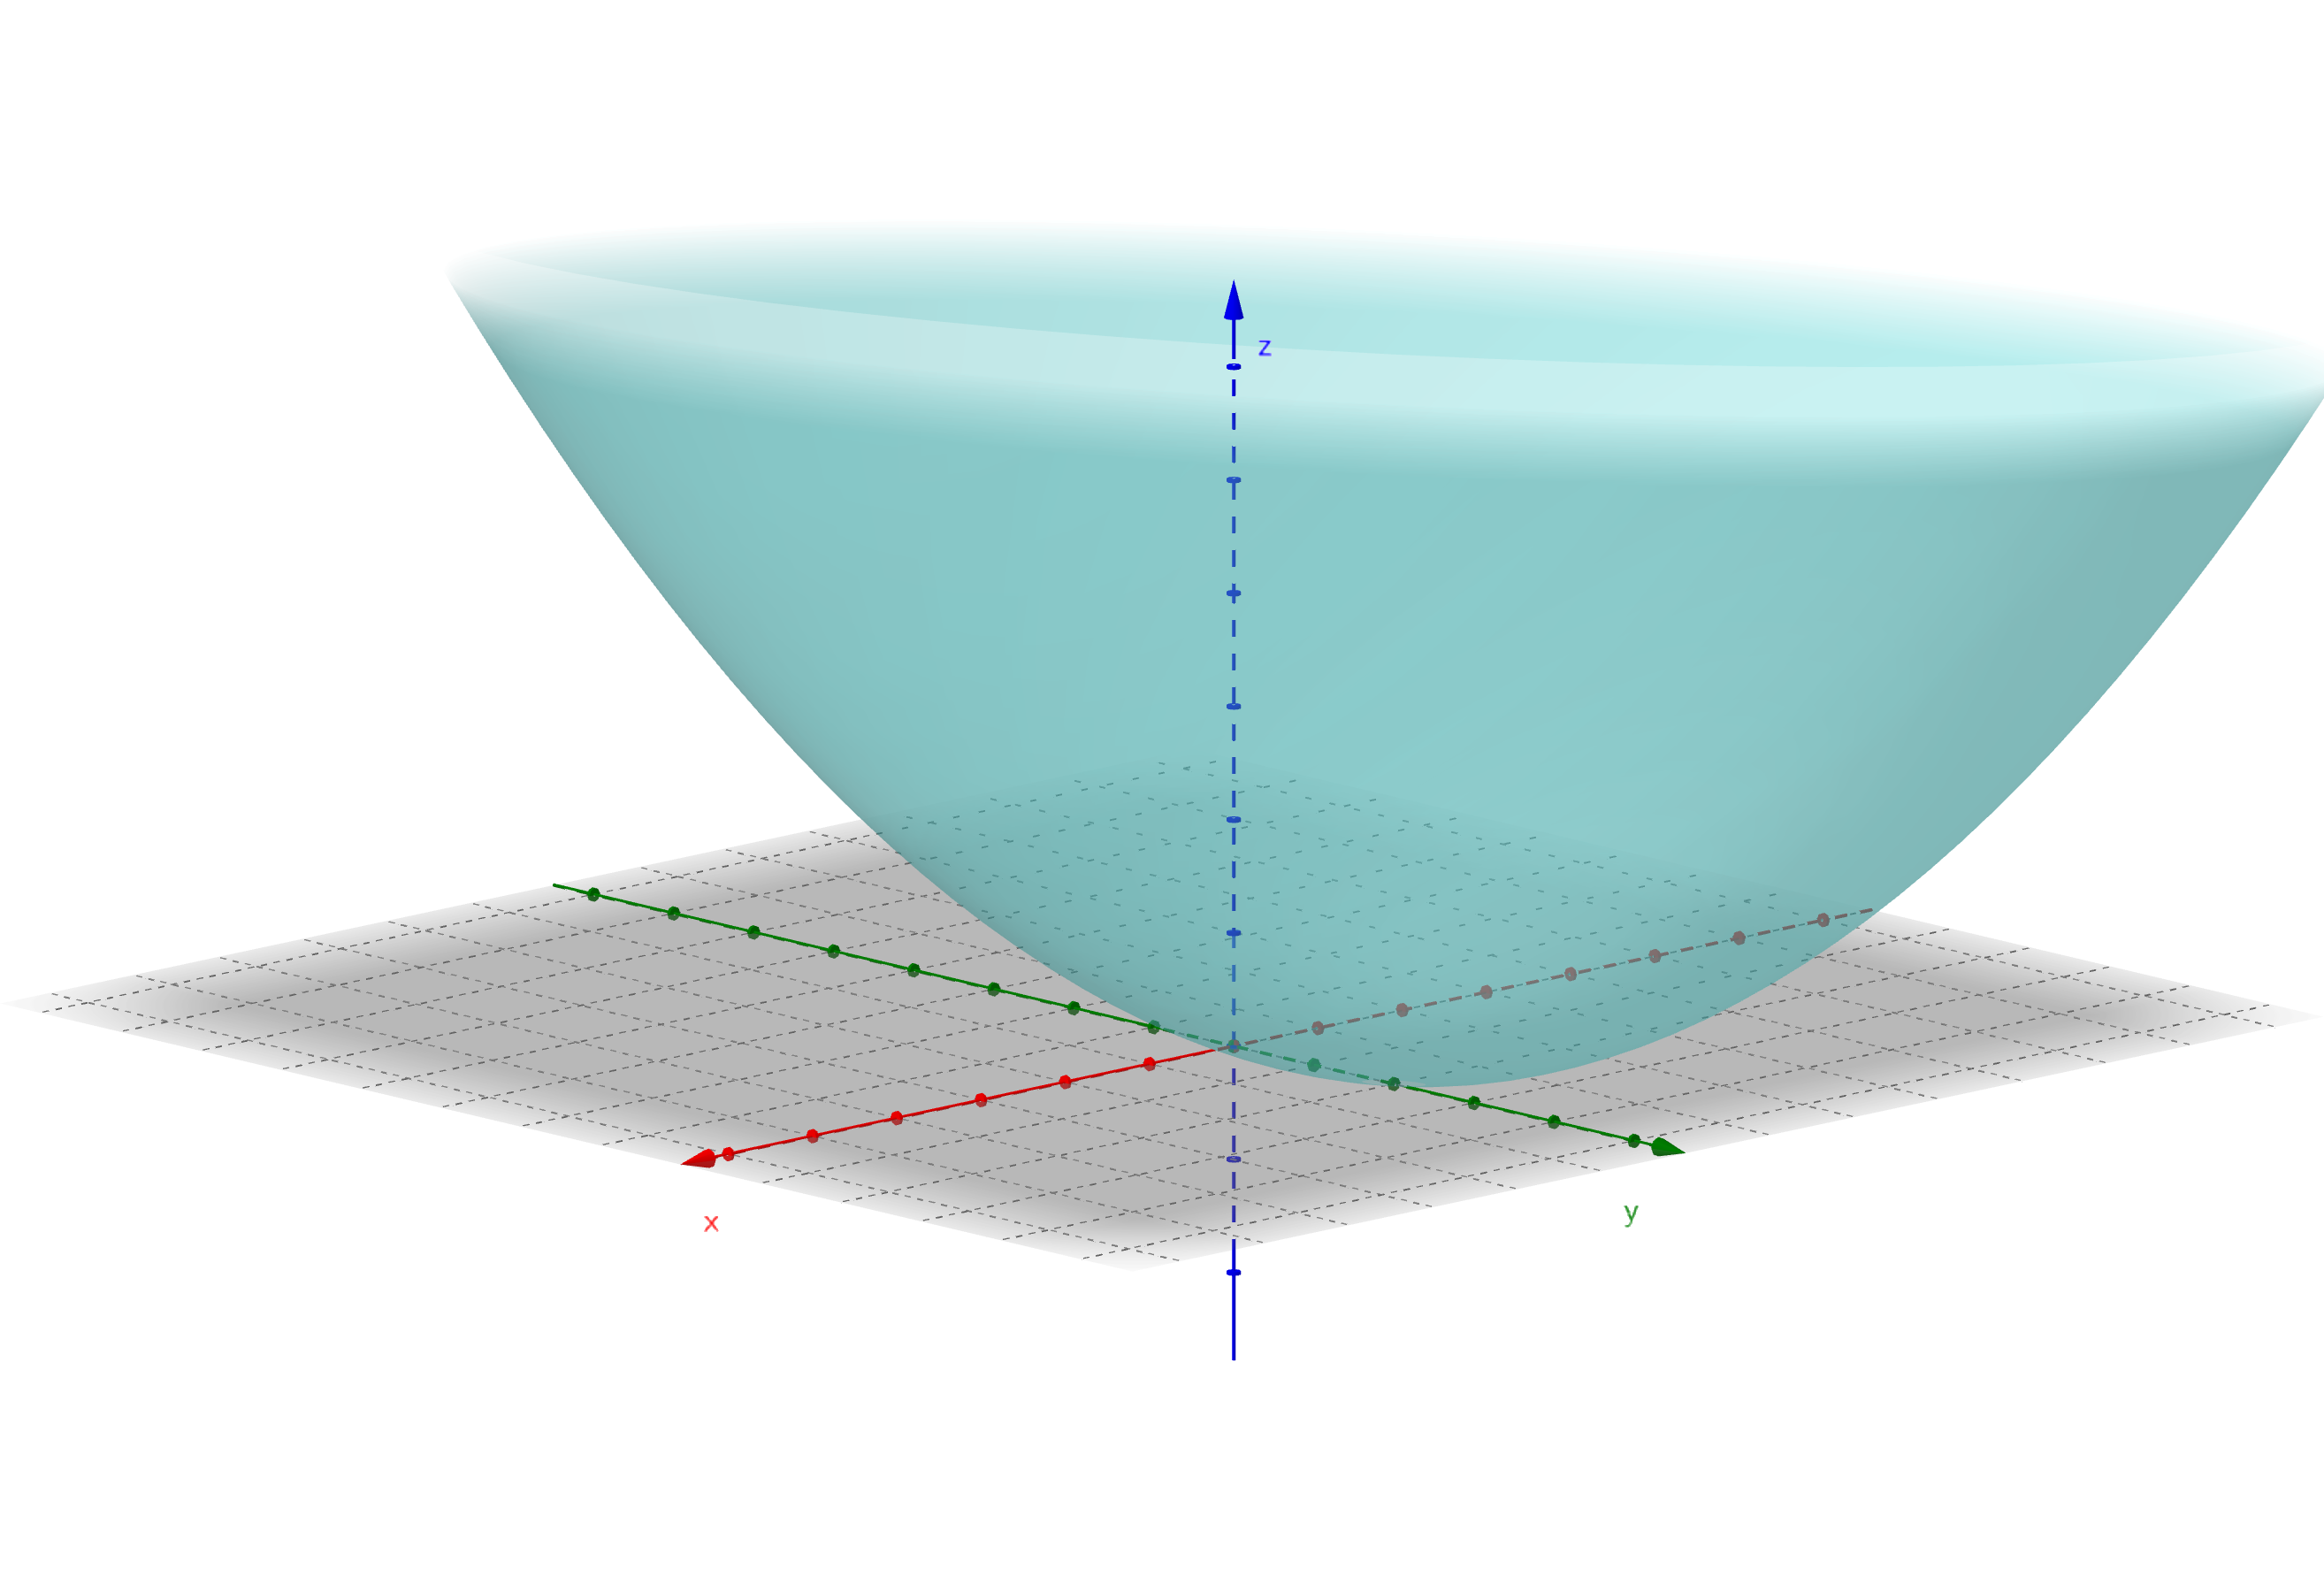
\includegraphics[width=0.5\textwidth]{bowl.png}
 \end{figure}
 


Level sets are sets of the form $L_{a}(f) = \set{x\st f(x)= a}$. 

\begin{figure}[h]
 \centering
  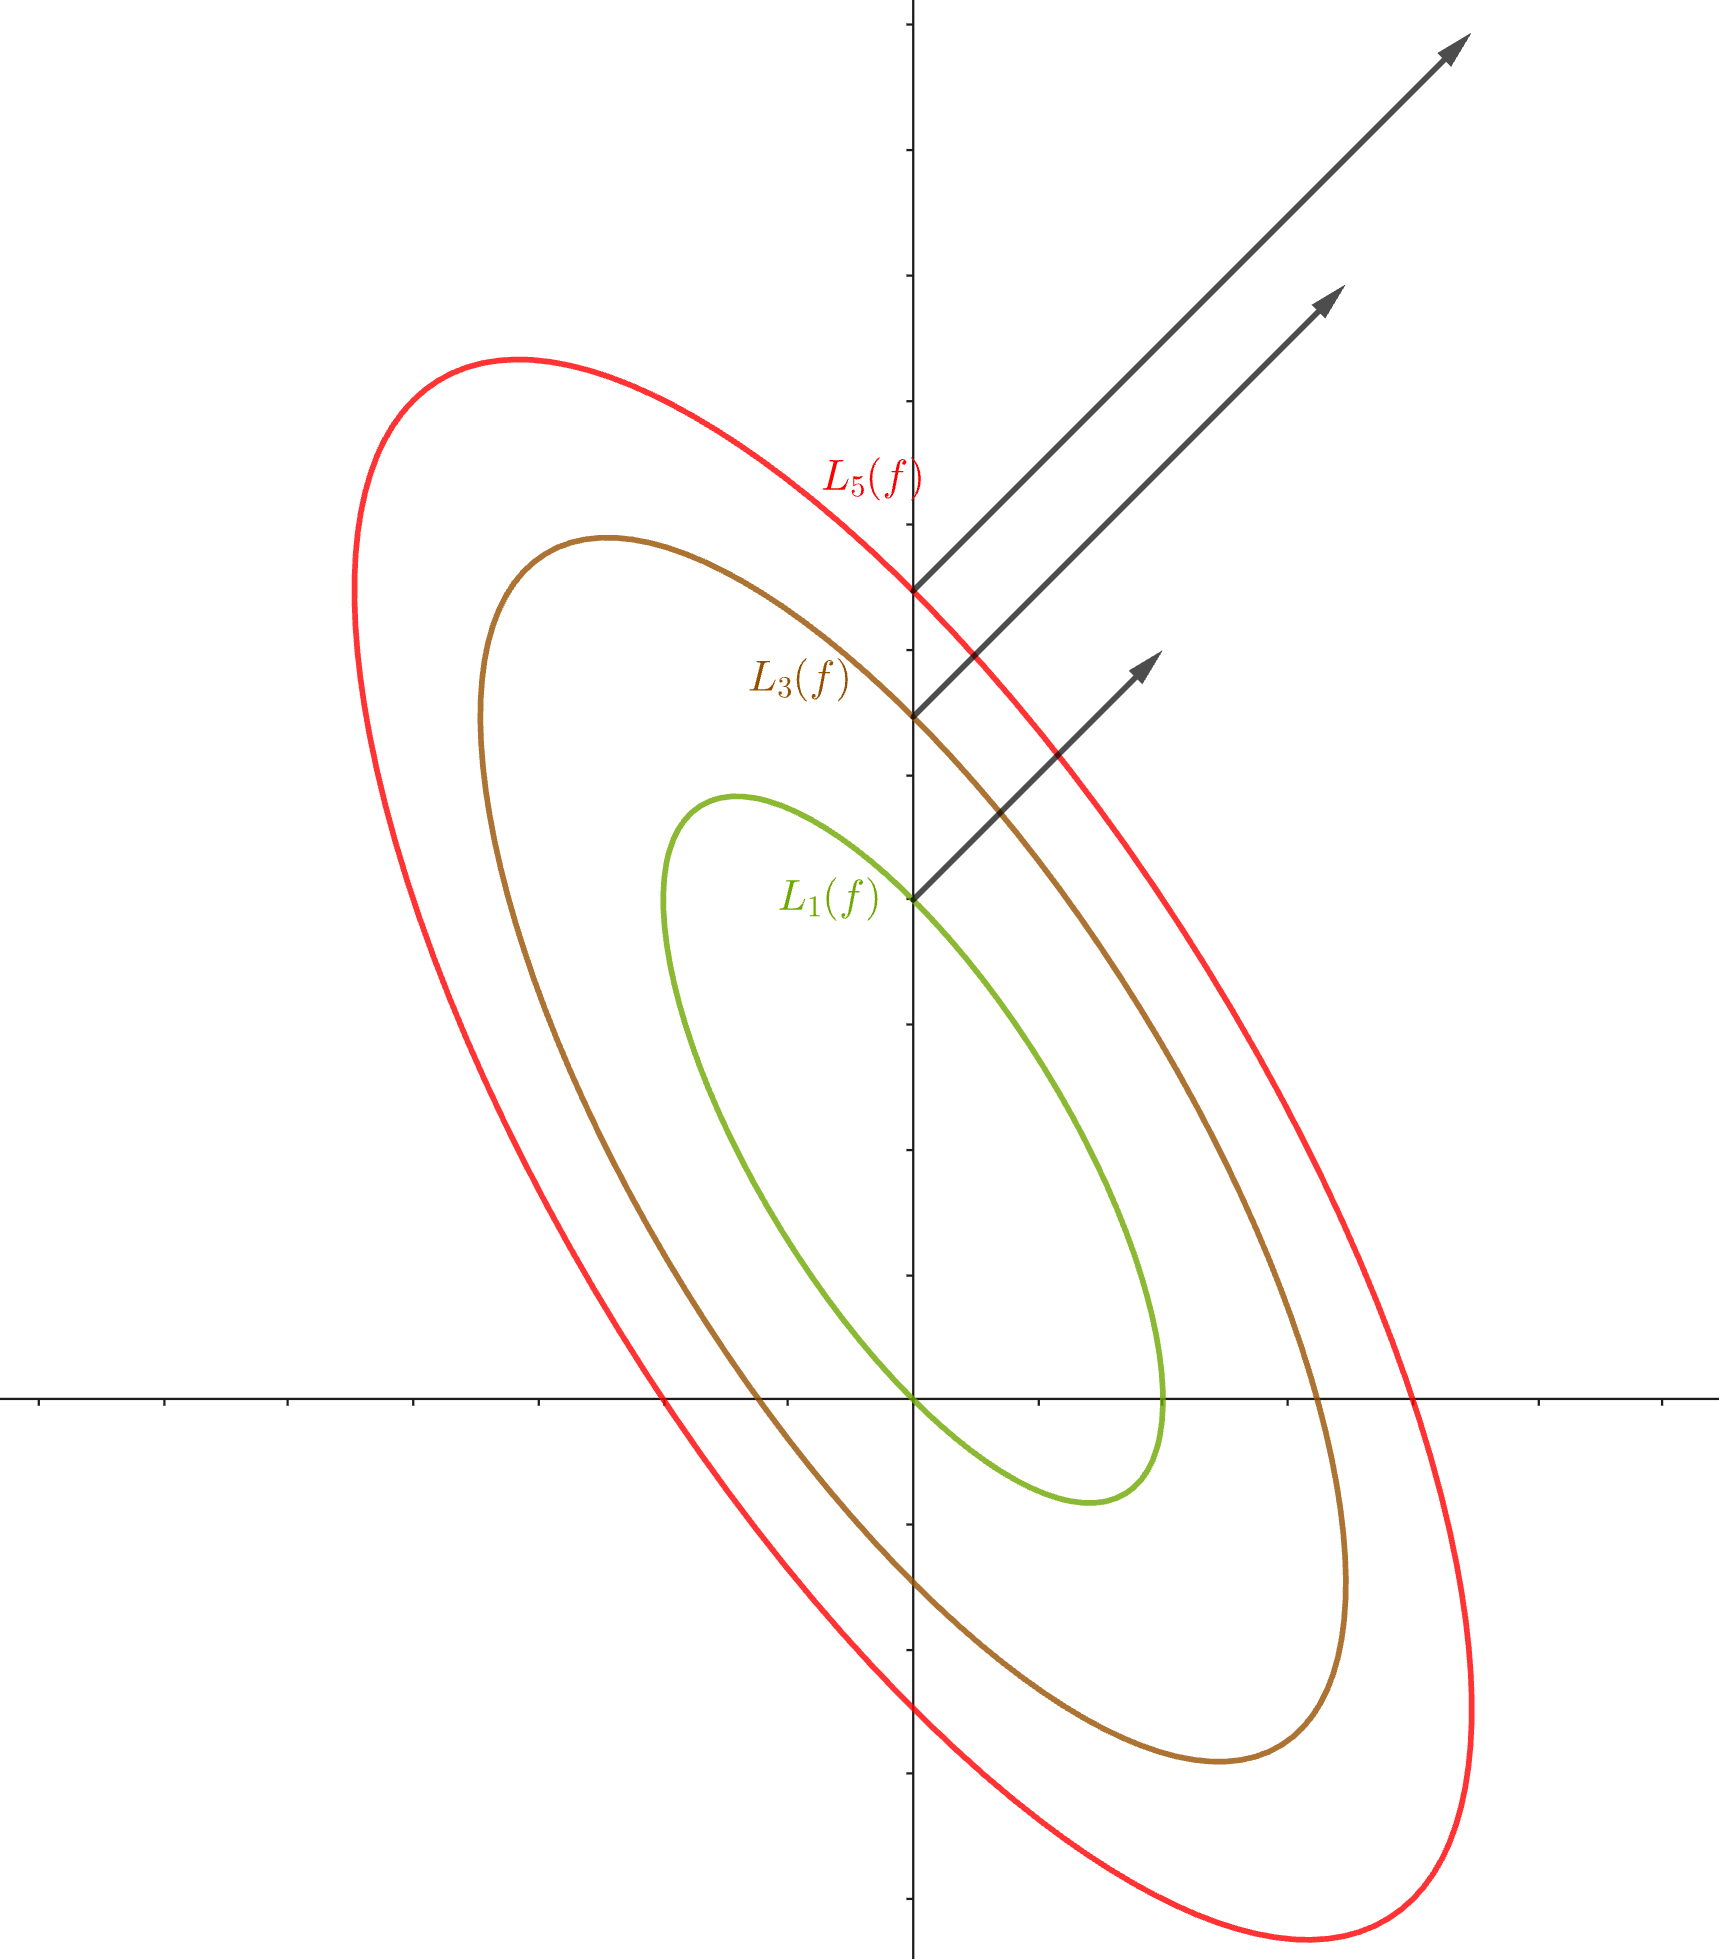
\includegraphics[width=0.5\textwidth]{level.png}
  \caption{Level sets $L_{a}(f)$ and the gradient vector at point $\left(0,1+\sqrt a\right)$ for $a=1,3,5$}
 \end{figure}

The gradient is $\nabla f(x) = \begin{bmatrix}
\frac{\partial f}{\partial x_{1}}\\
\frac{\partial f}{\partial x_{2}}
\end{bmatrix} = 
\begin{bmatrix}
2x_{1}+x_{2}-1\\x_{1}+x_{2}-1
\end{bmatrix}$.

The Hessian is $\nabla^{2}f(x) = \begin{bmatrix}
\partial_{11}f& \partial_{12}f\\
\partial_{21}f & \partial_{22}f
\end{bmatrix} = 
\begin{bmatrix}
2 & 1\\
1 & 1
\end{bmatrix}$. This is a symmetric matrix for $f\in \cC^{2}$, where $\cC^{2}$ is the class of twice differentiable functions with continuous second derivative.

We say a symmetric matrix $H$ is positive definite if $x^{\top}H x > 0 \fa x\ne 0$ and write $H\succ 0$.\\
We say a symmetric matrix $H$ is positive semi-definite if $x^{\top}H x \ge 0 \fa x$ and write $H\succeq 0$.

Why do we care about positive definiteness? Turns out that if $\nabla^{2}f\succ 0$ everywhere, then the function `looks like a cereal bowl'.

This Hessian also turns up in the objective of the $L^{2}$-regression. The objective is $
\frac12\norm{y-Ax}{}^{2} = \frac12 \left(y^{\top}-x^{\top}A^{\top}\right)\left( y-Ax \right)\\
= \frac12\left(\norm{y}{}^{2} - 2x^{\top}A^{\top}y  + x^{\top}A^{\top}Ax\right)\\
= \frac12 \left(\norm{y}{}^{2}-2x^{\top}A^{\top}y + x^{\top}\nabla^{2}f(x)x\right)
$

where we used the fact that $\nabla^{2} f(x) = A^{\top}A$ due to the absence of higher order terms and lower than second order terms are differentiated out to $0$. This also tells us that $\nabla f(x) = A^{\top}Ax-A^{\top}y$. If we are at a minima, then we set $\nabla f(x)=0$. This gives $x=\left(A^{\top}A\right)^{-1}A^{\top}y$ if $A^{\top}A$ is invertible. This has a couple of problems. $A^{\top}A$ is huge in the first place, and secondly, inverting a $d\times d$ matrix takes $\cO(d^{3})$ operations and we would like to have smaller computing time.


We have the following gradient descent algorithm: $x_{k+1} = x_{k} - \alpha_{k} \nabla f(x_{k})$. 

Let $\rho(H)$ denote the maximum (in absolute value) of $H$. We have the following theorem that will be stated rigorously and proved next day.

\begin{theorem}[informal]
Suppose $\nabla^{2}f(x)\succ 0$ and $\alpha_{k} \le \frac{2}{\rho\left(\nabla^{2}f(x)\right)}$, the above gradient descent algorithm converges `fast'. Otherwise it blows up. 
\end{theorem}















% ---------------------------
% References (optional)
% ---------------------------
%\begin{thebibliography}{9}

%\end{thebibliography}

\end{document}
